\documentclass[]{elsarticle} %review=doublespace preprint=single 5p=2 column
%%% Begin My package additions %%%%%%%%%%%%%%%%%%%
\usepackage[hyphens]{url}

  \journal{Journal of Archaeological Science} % Sets Journal name


\usepackage{lineno} % add
\providecommand{\tightlist}{%
  \setlength{\itemsep}{0pt}\setlength{\parskip}{0pt}}

\usepackage{graphicx}
\usepackage{booktabs} % book-quality tables
%%%%%%%%%%%%%%%% end my additions to header

\usepackage[T1]{fontenc}
\usepackage{lmodern}
\usepackage{amssymb,amsmath}
\usepackage{ifxetex,ifluatex}
\usepackage{fixltx2e} % provides \textsubscript
% use upquote if available, for straight quotes in verbatim environments
\IfFileExists{upquote.sty}{\usepackage{upquote}}{}
\ifnum 0\ifxetex 1\fi\ifluatex 1\fi=0 % if pdftex
  \usepackage[utf8]{inputenc}
\else % if luatex or xelatex
  \usepackage{fontspec}
  \ifxetex
    \usepackage{xltxtra,xunicode}
  \fi
  \defaultfontfeatures{Mapping=tex-text,Scale=MatchLowercase}
  \newcommand{\euro}{€}
\fi
% use microtype if available
\IfFileExists{microtype.sty}{\usepackage{microtype}}{}
\bibliographystyle{elsarticle-harv}
\usepackage{longtable}
\usepackage{graphicx}
\ifxetex
  \usepackage[setpagesize=false, % page size defined by xetex
              unicode=false, % unicode breaks when used with xetex
              xetex]{hyperref}
\else
  \usepackage[unicode=true]{hyperref}
\fi
\hypersetup{breaklinks=true,
            bookmarks=true,
            pdfauthor={},
            pdftitle={},
            colorlinks=false,
            urlcolor=blue,
            linkcolor=magenta,
            pdfborder={0 0 0}}
\urlstyle{same}  % don't use monospace font for urls

\setcounter{secnumdepth}{5}
% Pandoc toggle for numbering sections (defaults to be off)

% Pandoc citation processing
\newlength{\csllabelwidth}
\setlength{\csllabelwidth}{3em}
\newlength{\cslhangindent}
\setlength{\cslhangindent}{1.5em}
% for Pandoc 2.8 to 2.10.1
\newenvironment{cslreferences}%
  {}%
  {\par}
% For Pandoc 2.11+
\newenvironment{CSLReferences}[3] % #1 hanging-ident, #2 entry sp
 {% don't indent paragraphs
  \setlength{\parindent}{0pt}
  % turn on hanging indent if param 1 is 1
  \ifodd #1 \everypar{\setlength{\hangindent}{\cslhangindent}}\ignorespaces\fi
  % set line spacing
  % set entry spacing
  \ifnum #2 > 0
  \setlength{\parskip}{#3\baselineskip}
  \fi
 }%
 {}
\usepackage{calc} % for \widthof, \maxof
\newcommand{\CSLBlock}[1]{#1\hfill\break}
\newcommand{\CSLLeftMargin}[1]{\parbox[t]{\maxof{\widthof{#1}}{\csllabelwidth}}{#1}}
\newcommand{\CSLRightInline}[1]{\parbox[t]{\linewidth}{#1}}
\newcommand{\CSLIndent}[1]{\hspace{\cslhangindent}#1}

% Pandoc header



\begin{document}
\begin{frontmatter}

  \title{}
    \author[Some Institute of Technology]{Alice Anonymous\corref{1}}
   \ead{alice@example.com} 
    \author[Another University]{Bob Security}
   \ead{bob@example.com} 
    \author[Another University]{Cat Memes\corref{2}}
   \ead{cat@example.com} 
    \author[Some Institute of Technology]{Derek Zoolander\corref{2}}
   \ead{derek@example.com} 
      \address[Some Institute of Technology]{Department, Street, City, State, Zip}
    \address[Another University]{Department, Street, City, State, Zip}
      \cortext[1]{Corresponding Author}
    \cortext[2]{Equal contribution}
  
  \begin{abstract}
  This is the abstract.

  It consists of two paragraphs.
  \end{abstract}
  
 \end{frontmatter}

Keywords:

Highlights:

\hypertarget{introduction}{%
\section{Introduction}\label{introduction}}

Here is a citation (Marwick, 2017)

\hypertarget{background}{%
\section{Background}\label{background}}

\hypertarget{methods}{%
\section{Methods}\label{methods}}

\hypertarget{results}{%
\section{Results}\label{results}}

\begin{figure}
\centering
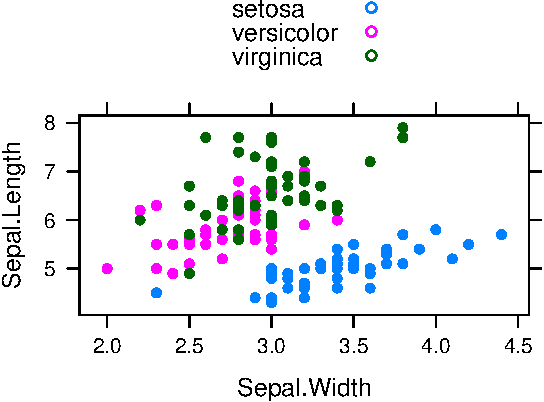
\includegraphics{../figures/demo-plot-1.pdf}
\caption{\label{fig:demo-plot}A plot of iris data}
\end{figure}

Figure \ref{fig:demo-plot} shows how we can have a caption and cross-reference for a plot

Corresponding p-value: 0.001.

\hypertarget{discussion}{%
\section{Discussion}\label{discussion}}

\hypertarget{conclusion}{%
\section{Conclusion}\label{conclusion}}

\hypertarget{acknowledgements}{%
\section{Acknowledgements}\label{acknowledgements}}

\newpage

\hypertarget{references}{%
\section{References}\label{references}}

\hypertarget{refs}{}
\begin{CSLReferences}{1}{0}
\leavevmode\hypertarget{ref-Marwick2017}{}%
Marwick, B., 2017. Computational reproducibility in archaeological research: Basic principles and a case study of their implementation. Journal of Archaeological Method and Theory 24, 424--450. \url{https://doi.org/10.1007/s10816-015-9272-9}

\end{CSLReferences}

\newpage

\hypertarget{colophon}{%
\subsubsection{Colophon}\label{colophon}}

This report was generated on 2020-12-07 15:10:52 using the following computational environment and dependencies:

\begin{verbatim}
#> - Session info -------------------------------------------
#>  setting  value                       
#>  version  R version 4.0.3 (2020-10-10)
#>  os       Manjaro Linux               
#>  system   x86_64, linux-gnu           
#>  ui       X11                         
#>  language (EN)                        
#>  collate  fr_FR.UTF-8                 
#>  ctype    fr_FR.UTF-8                 
#>  tz       Europe/Paris                
#>  date     2020-12-07                  
#> 
#> - Packages -----------------------------------------------
#>  package     * version date       lib source        
#>  assertthat    0.2.1   2019-03-21 [1] CRAN (R 4.0.0)
#>  bookdown      0.21    2020-10-13 [1] CRAN (R 4.0.2)
#>  callr         3.5.1   2020-10-13 [1] CRAN (R 4.0.2)
#>  cli           2.2.0   2020-11-20 [1] CRAN (R 4.0.3)
#>  cluster       2.1.0   2019-06-19 [1] CRAN (R 4.0.0)
#>  crayon        1.3.4   2017-09-16 [1] CRAN (R 4.0.0)
#>  desc          1.2.0   2018-05-01 [1] CRAN (R 4.0.0)
#>  devtools      2.3.2   2020-09-18 [1] CRAN (R 4.0.2)
#>  digest        0.6.27  2020-10-24 [1] CRAN (R 4.0.2)
#>  ellipsis      0.3.1   2020-05-15 [1] CRAN (R 4.0.0)
#>  evaluate      0.14    2019-05-28 [1] CRAN (R 4.0.0)
#>  fansi         0.4.1   2020-01-08 [1] CRAN (R 4.0.0)
#>  fs            1.5.0   2020-07-31 [1] CRAN (R 4.0.2)
#>  glue          1.4.2   2020-08-27 [1] CRAN (R 4.0.2)
#>  here          1.0.0   2020-11-15 [1] CRAN (R 4.0.3)
#>  highr         0.8     2019-03-20 [1] CRAN (R 4.0.0)
#>  htmltools     0.5.0   2020-06-16 [1] CRAN (R 4.0.1)
#>  knitr         1.30    2020-09-22 [1] CRAN (R 4.0.2)
#>  lattice       0.20-41 2020-04-02 [2] CRAN (R 4.0.3)
#>  magrittr      2.0.1   2020-11-17 [1] CRAN (R 4.0.3)
#>  MASS          7.3-53  2020-09-09 [1] CRAN (R 4.0.2)
#>  Matrix        1.2-18  2019-11-27 [2] CRAN (R 4.0.3)
#>  memoise       1.1.0   2017-04-21 [1] CRAN (R 4.0.0)
#>  mgcv          1.8-33  2020-08-27 [1] CRAN (R 4.0.2)
#>  nlme          3.1-150 2020-10-24 [1] CRAN (R 4.0.2)
#>  permute       0.9-5   2019-03-12 [1] CRAN (R 4.0.0)
#>  pkgbuild      1.1.0   2020-07-13 [1] CRAN (R 4.0.2)
#>  pkgload       1.1.0   2020-05-29 [1] CRAN (R 4.0.0)
#>  prettyunits   1.1.1   2020-01-24 [1] CRAN (R 4.0.0)
#>  processx      3.4.5   2020-11-30 [1] CRAN (R 4.0.3)
#>  ps            1.5.0   2020-12-05 [1] CRAN (R 4.0.3)
#>  R6            2.5.0   2020-10-28 [1] CRAN (R 4.0.2)
#>  remotes       2.2.0   2020-07-21 [1] CRAN (R 4.0.2)
#>  rlang         0.4.9   2020-11-26 [1] CRAN (R 4.0.3)
#>  rmarkdown     2.5     2020-10-21 [1] CRAN (R 4.0.2)
#>  rprojroot     2.0.2   2020-11-15 [1] CRAN (R 4.0.3)
#>  rticles       0.17    2020-11-01 [1] CRAN (R 4.0.2)
#>  sessioninfo   1.1.1   2018-11-05 [1] CRAN (R 4.0.0)
#>  stringi       1.5.3   2020-09-09 [1] CRAN (R 4.0.2)
#>  stringr       1.4.0   2019-02-10 [1] CRAN (R 4.0.0)
#>  testthat      3.0.0   2020-10-31 [1] CRAN (R 4.0.2)
#>  usethis       1.6.3   2020-09-17 [1] CRAN (R 4.0.2)
#>  vegan         2.5-7   2020-11-28 [1] CRAN (R 4.0.3)
#>  withr         2.3.0   2020-09-22 [1] CRAN (R 4.0.2)
#>  xfun          0.19    2020-10-30 [1] CRAN (R 4.0.2)
#>  yaml          2.2.1   2020-02-01 [1] CRAN (R 4.0.0)
#> 
#> [1] /home/fsantos/R/x86_64-pc-linux-gnu-library/4.0
#> [2] /usr/lib/R/library
\end{verbatim}

The current Git commit details are:

\begin{verbatim}
#> Local:    master /home/fsantos/PACEA_MyCore/Perso_work/fakepaper
#> Head:     [606e08c] 2020-12-07: Première version avec le template
\end{verbatim}


\end{document}

